\section{Experiment 10C: backbone-to-personalization transition}
\label{sec:experiment10c}

\paragraph{Purpose.}
Experiment 10B showed that complementary oracle-family sharing solves the
restricted-coverage identification problem, but that immediate personalization
is worse than the shared family backbone. Experiment 10C asks whether this is a
cold-start effect: as a recipient covers more of the speed envelope, does a
client-specific head eventually become useful, and does any model improvement
translate into control performance?

This experiment is a development sweep, not a confirmation run. Its purpose is
to determine which estimator structure deserves a federated implementation.
The result may support a staged backbone-to-personalization policy, a permanently
shared family model, or a transition directly from the family model to Local.

\paragraph{Frozen and progressive information.}
Ten fresh fleets, seeds 341--350, use the 10B plant, excitation, noise,
curvature, $L=7$ basis, and nonlinear recovery test. Initial speed-block
assignment is balanced independently inside each oracle family; hence every
family jointly covers all four blocks. The FamilyPool backbone is fit once from
the initial client blocks and then frozen.

Each recipient starts with its original two- or three-speed block, averaging
2.8 speeds and 100.8 transitions. It then adds the nearest missing speeds until
covering 5, 8, and all 11 grid speeds. These stages contain 180, 288, and 396
local transitions. The added recipient records never update FamilyPool. This
separates a fixed fleet prior from increasing client information.

The comparison contains four models. FamilyPool is the fixed oracle-family
backbone. FamilyPersonalized fits an $L=7$ client model around that backbone,
with ridge strength selected by leave-one-local-speed-out validation.
LocalRegularized uses the same local records but an $L=3$ locally estimated
physics prior instead of fleet knowledge. ExactLPV remains the exact-Jacobian
reference. Metrics cover the complete speed envelope at every stage, including
the locally measured speeds.

\paragraph{Safety guard.}
Personalization must not sacrifice deployability. If a personalized controller
fails the nonlinear recovery feasibility check, deployment falls back to the
FamilyPool controller at that speed. An infeasible LocalRegularized controller
falls back to its nearest-observed-speed $L=3$ physics controller. Every fallback
is recorded. This guard prevents unsafe adaptation from appearing as an
accuracy improvement and distinguishes nominal estimator quality from the
deployed safe policy.

\paragraph{Statistical criterion.}
At each stage, paired differences are formed after averaging all clients and
speeds within each fleet. A crossover is declared only when the 95\% bootstrap
interval of the mean improvement over FamilyPool is positive. Prediction and
control crossovers are tested separately; a personalized-control claim requires
both. As in 10B, 20000 resamples use the ten fleets as independent units.

\begin{table}[htbp]
\centering
\caption{Experiment 10C full-envelope results. Errors are percentages;
recovery is normalized nonlinear RMS.}
\label{tab:experiment10c-summary}
\begin{tabular}{rrrrrrrr}
\toprule
Speeds & Trans. & \multicolumn{2}{c}{FamilyPool} &
\multicolumn{2}{c}{Personalized} & \multicolumn{2}{c}{Local}\\
 & & Error & Recovery & Error & Recovery & Error & Recovery\\
\midrule
2.8 & 100.8 & 1.631 & 0.17671 & 1.717 & 0.17676 & 43.694 & 0.19585\\
5   & 180   & 1.631 & 0.17671 & 1.656 & 0.17679 & 13.392 & 0.18265\\
8   & 288   & 1.631 & 0.17671 & 1.505 & 0.17676 & 2.565  & 0.17755\\
11  & 396   & 1.631 & 0.17671 & 1.406 & 0.17672 & 1.236  & 0.17675\\
\bottomrule
\end{tabular}
\end{table}

\begin{figure}[htbp]
\centering
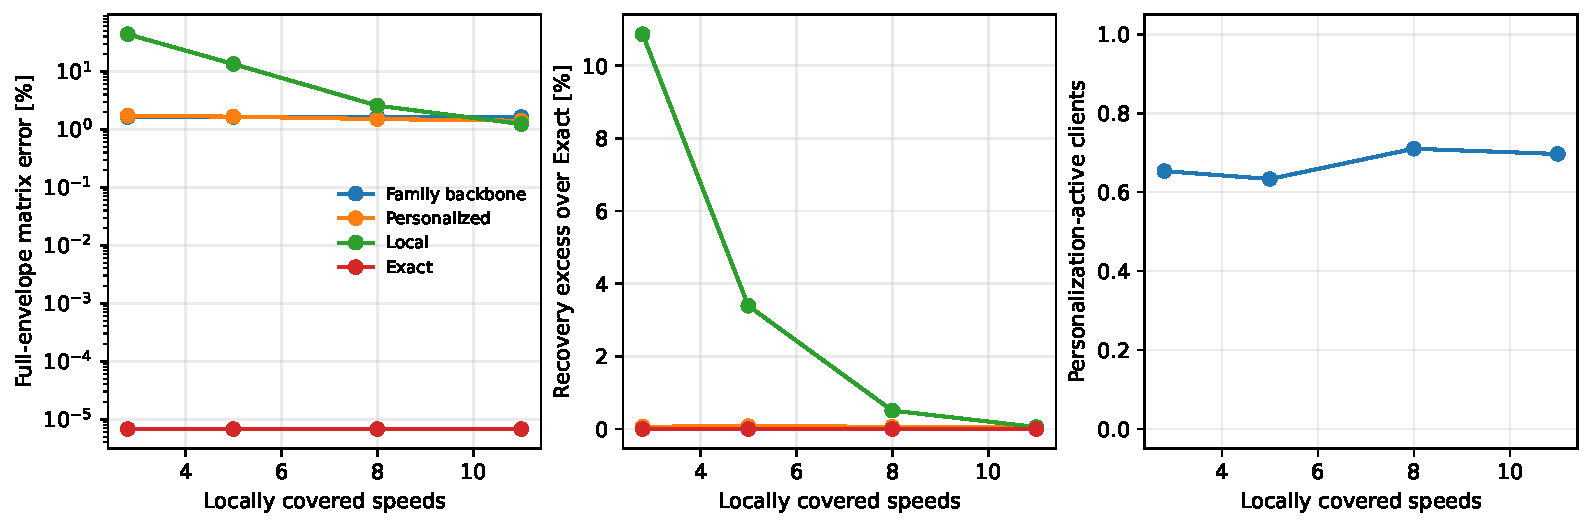
\includegraphics[width=0.98\linewidth]{../results/figures/experiment_10c_personalization_transition.pdf}
\caption{Full-envelope identification, recovery excess over ExactLPV, and the
fraction of clients whose validation-selected personalization strength does not
exceed one. Personalization improves model quality only after sufficient speed
coverage and never improves recovery over the backbone.}
\label{fig:experiment10c}
\end{figure}

\begin{table}[htbp]
\centering
\caption{FamilyPersonalized relative to the fixed FamilyPool. Positive values
favor personalization.}
\label{tab:experiment10c-comparisons}
\begin{tabular}{rrlrrr}
\toprule
Speeds & Trans. & Metric & Mean & 95\% CI & Wins\\
\midrule
2.8 & 100.8 & Prediction & -5.37\% & [-7.31,-3.57]\% & 0/10\\
2.8 & 100.8 & Recovery   & -0.030\% & [-0.050,-0.014]\% & 1/10\\
5   & 180   & Prediction & -1.61\% & [-3.93,0.77]\% & 4/10\\
5   & 180   & Recovery   & -0.047\% & [-0.079,-0.018]\% & 2/10\\
8   & 288   & Prediction & 7.74\% & [5.69,10.01]\% & 10/10\\
8   & 288   & Recovery   & -0.030\% & [-0.072,-0.004]\% & 1/10\\
11  & 396   & Prediction & 13.66\% & [10.62,16.81]\% & 10/10\\
11  & 396   & Recovery   & -0.006\% & [-0.020,0.008]\% & 5/10\\
\bottomrule
\end{tabular}
\end{table}

\paragraph{Identification transition.}
At cold start, personalization is significantly worse than FamilyPool by
5.37\%. Five covered speeds are still insufficient to resolve an advantage.
The first reliable prediction crossover occurs at eight speeds: personalization
improves full-envelope error by 7.74\%, with a [5.69,10.01]\% interval and wins
all ten fleets. At full coverage the improvement grows to 13.66\% and again
wins every fleet. The shared backbone therefore becomes a useful prior for
client adaptation once local data span most of the scheduling envelope.

The locally selected ridge strength alone does not provide a trustworthy
activation rule. Between 63\% and 71\% of clients are classified as active at
all stages, including cold start where personalization is harmful. A deployment
rule must therefore incorporate coverage or aggregate information rank rather
than relying only on local validation loss.

\paragraph{Control result.}
There is no control crossover. Personalization is slightly but significantly
worse at two, five, and eight covered speeds. At full coverage it reaches parity
with FamilyPool: the mean difference is $-0.006\%$ with a
$[-0.020,0.008]\%$ interval. Feedback suppresses the model-quality differences
that are clear in open-loop matrix error. All guarded personalized evaluations
are feasible; fallback is required for only $0.030\%$ of evaluations at the
five-speed stage and never at the other stages.

LocalRegularized provides a second boundary. It is unusable without its safety
fallback at low coverage, but at all eleven speeds it becomes the most accurate
finite-data model: 1.236\% error versus 1.406\% for FamilyPersonalized. It is
13.79\% more accurate than personalization with a confidence interval bounded
away from zero, while their recovery remains statistically equivalent. Thus the
eventual endpoint is fully local identification, not indefinite personalization.

\paragraph{Decision.}
Experiment 10C supports a three-stage identification policy:
\begin{enumerate}
 \item use the compatible shared backbone at cold start;
 \item enable a personalized head only after broad local scheduling coverage,
 with eight of eleven speeds as the observed development crossover;
 \item switch to a fully local $L=7$ model once full-envelope local data are
 available.
\end{enumerate}
This policy is supported for model accuracy, not for improved closed-loop
recovery. The paper should therefore frame personalization as progressive model
ownership and local fidelity, while the demonstrated control advantage remains
the approximately 1.7\% gain of complementary sharing over the conservative
restricted Local controller from 10B.

The next experiment should replace oracle family labels with learned compatible
groups while retaining FamilyPool as the cold-start anchor and the coverage
gate for personalization. Only after that test should the aggregation be
implemented federatively.

\paragraph{Reproducibility.}
The configuration and implementation are in
\path{code/config/experiment_10c.json} and
\path{code/experiments/experiment_10c_personalization_transition.py}. Per-fleet
records, fit diagnostics, fallback rates, aggregate summaries, paired bootstrap
comparisons, and provenance hashes are stored under \path{results/tables}.
